\documentclass[
	%sans,			% use sans-serif font
	%serif,			% use serif-font
	%mathsans,		% set mathtext to sans-serif
	%mathserif,		% set mathtext to serif
	%10pt,
	10pt,
	%12pt,
	t		% add text at the top border of slide
	%slidescentered,% center text on slide
	%draft,			% compile as draft version
	%handout,		% create handout file
	%notes,			% include nodes in slides
	%compress		% compress navigation bar
]{beamer}


\usetheme{lmtslides}
\usepackage{eso-pic}
\usepackage{graphicx}
%\usepackage[pdftex]{color}
\usepackage{times}
\usepackage[latin1]{inputenc}
%\usepackage[T1]{fontenc}
\usepackage[amssymb]{SIunits}
\usepackage{amsmath,amssymb}
\usepackage{eurosym}
\usepackage{booktabs}
\usepackage{colortbl}
\usepackage{url}

\graphicspath{{figures/}}

% SET LANGUAGE HERE! (Babel is already included and setup by this call.)
\setlang{de}		% <- GERMAN
%\setlang{en}		% <- ENGLISH

% MODIFY THESE ACCORDINGLY! ---
\title{Mancala}
\subtitle{}
\type{Xml} % (M/B/D/S)(f/m): (Master/Bachelor/Diplom/Studienarbeit)(final/midterm)
\advisor{Team XML Schema}
\author{Michael Conrads \\ Andreas Eichner \\ Emiliyana Kalinova \\ Nean Nguyen \\ Son Nguyen}
\date{01. Juli 2016}
%------------------------------


%%%%%%%%%%%%%%%%%%%%%%%%%%
\begin{document}

\AddToShipoutPicture{\TitlePicture}
\maketitle
\ClearShipoutPicture
\AddToShipoutPicture{\BackgroundPicture}

\section{Outline}
\begin{frame}
\frametitle{Outline}
\begin{enumerate}
\item Mancala
\item Technologien
\item Architektur
\item UML
\item Demo
\item Probleme
\end{enumerate}
\end{frame}

\section{Mancala}
\begin{frame}
\frametitle{Outline}
\begin{enumerate}
\item \textbf{Mancala}
\item Technologien
\item Architektur
\item UML
\item Demo
\item Probleme
\end{enumerate}
\end{frame}

\begin{frame}
\frametitle{Mancala}

\end{frame}

\section{Technologies}
\begin{frame}
\frametitle{Outline}
\begin{enumerate}
\item Mancala
\item \textbf{Technologien}
\item Architektur
\item UML
\item Demo
\item Probleme
\end{enumerate}
\end{frame}

\begin{frame}
\frametitle{Technologien}

\end{frame}

\section{Architecture}
\begin{frame}
\frametitle{Outline}
\begin{enumerate}
\item Mancala
\item Technologien
\item \textbf{Architektur}
\item UML
\item Demo
\item Probleme
\end{enumerate}
\end{frame}

\begin{frame}
\frametitle{Architektur}

\end{frame}

\section{UML}
\begin{frame}
\frametitle{Outline}
\begin{enumerate}
\item Mancala
\item Technologien
\item Architektur
\item \textbf{UML}
\item Demo
\item Probleme
\end{enumerate}
\end{frame}

\begin{frame}
\frametitle{Outline}
\begin{enumerate}
\item Mancala
\item Technologien
\item Architektur
\item \textbf{UML}
\begin{enumerate}
\item Anwendungsfalldiagram
\item Sequenzdiagram
\item Klassendiagram
\end{enumerate}
\item Demo
\item Probleme
\end{enumerate}
\end{frame}

\subsection{Use Case Diagram}
\begin{frame}
\frametitle{Outline}
\begin{enumerate}
\item Mancala
\item Technologien
\item Architektur
\item UML
\begin{enumerate}
\item \textbf{Anwendungsfalldiagram}
\item Sequenzdiagram
\item Klassendiagram
\end{enumerate}
\item Demo
\item Probleme
\end{enumerate}
\end{frame}

\begin{frame}
\frametitle{Anwendungsfalldiagram}
\begin{center}
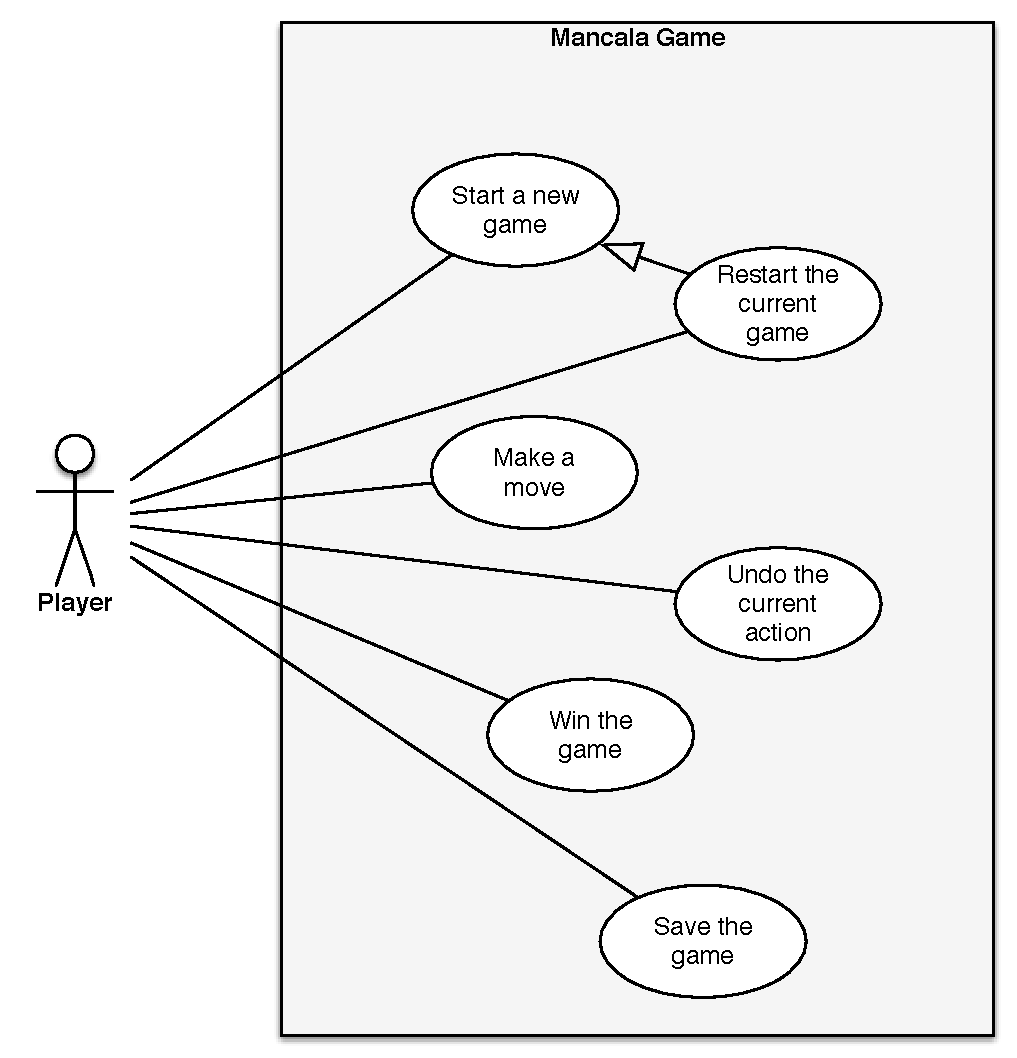
\includegraphics[scale=0.32]{./../Diagrams/UseCaseDiagram.pdf}
\end{center}
\end{frame}

\subsection{Sequenz Diagram}
\begin{frame}
\frametitle{Outline}
\begin{enumerate}
\item Mancala
\item Technologien
\item Architektur
\item UML
\begin{enumerate}
\item Anwendungsfalldiagram
\item \textbf{Sequenzdiagram}
\item Klassendiagram
\end{enumerate}
\item Demo
\item Probleme
\end{enumerate}
\end{frame}

\begin{frame}
\frametitle{Sequenzdiagram}
\begin{center}
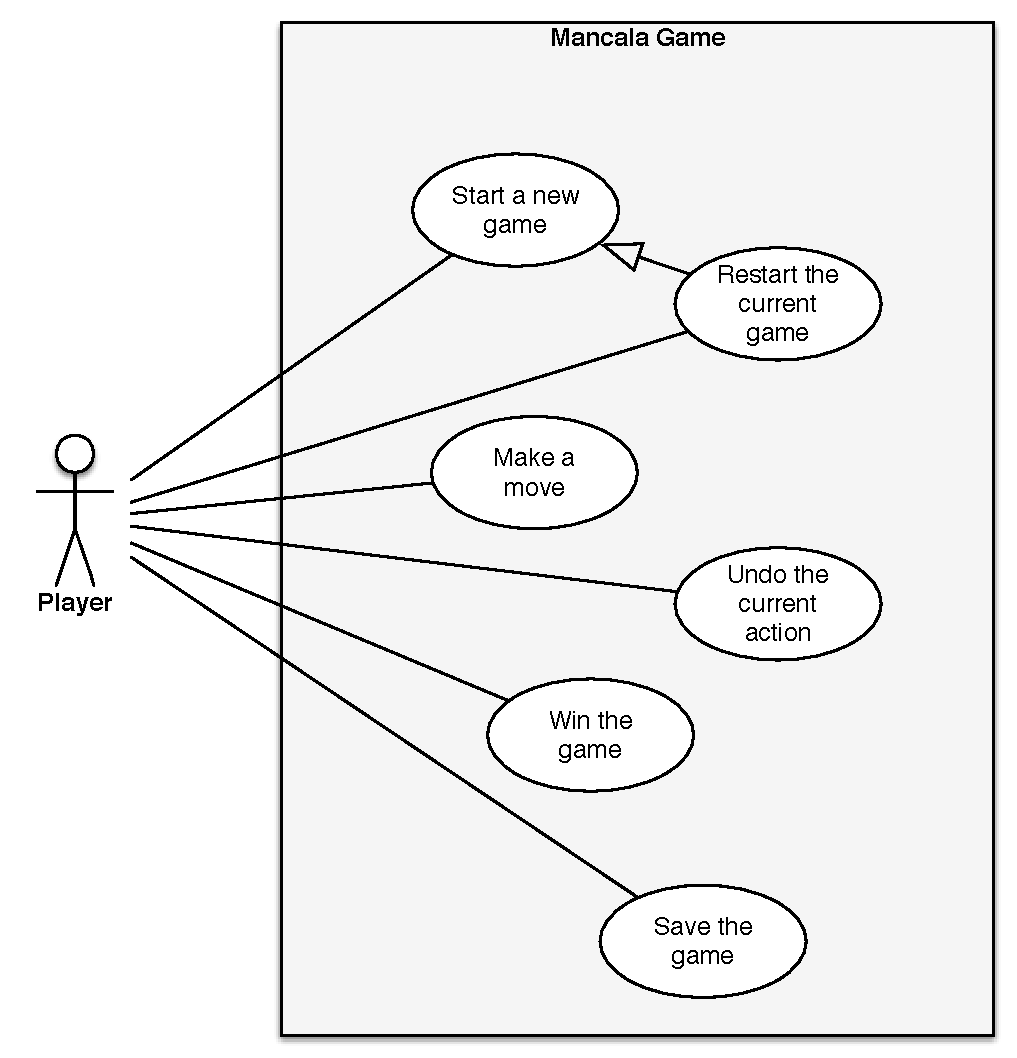
\includegraphics[scale=0.32]{./../Diagrams/SequenzDiagram.pdf}
\end{center}
\end{frame}

\subsection{Class Diagram}
\begin{frame}
\frametitle{Outline}
\begin{enumerate}
\item Mancala
\item Technologien
\item Architektur
\item UML
\begin{enumerate}
\item Anwendungsfalldiagram
\item Sequenzdiagram
\item \textbf{Klassendiagram}
\end{enumerate}
\item Demo
\item Probleme
\end{enumerate}
\end{frame}

\begin{frame}
\frametitle{Klassendiagram}
\begin{center}
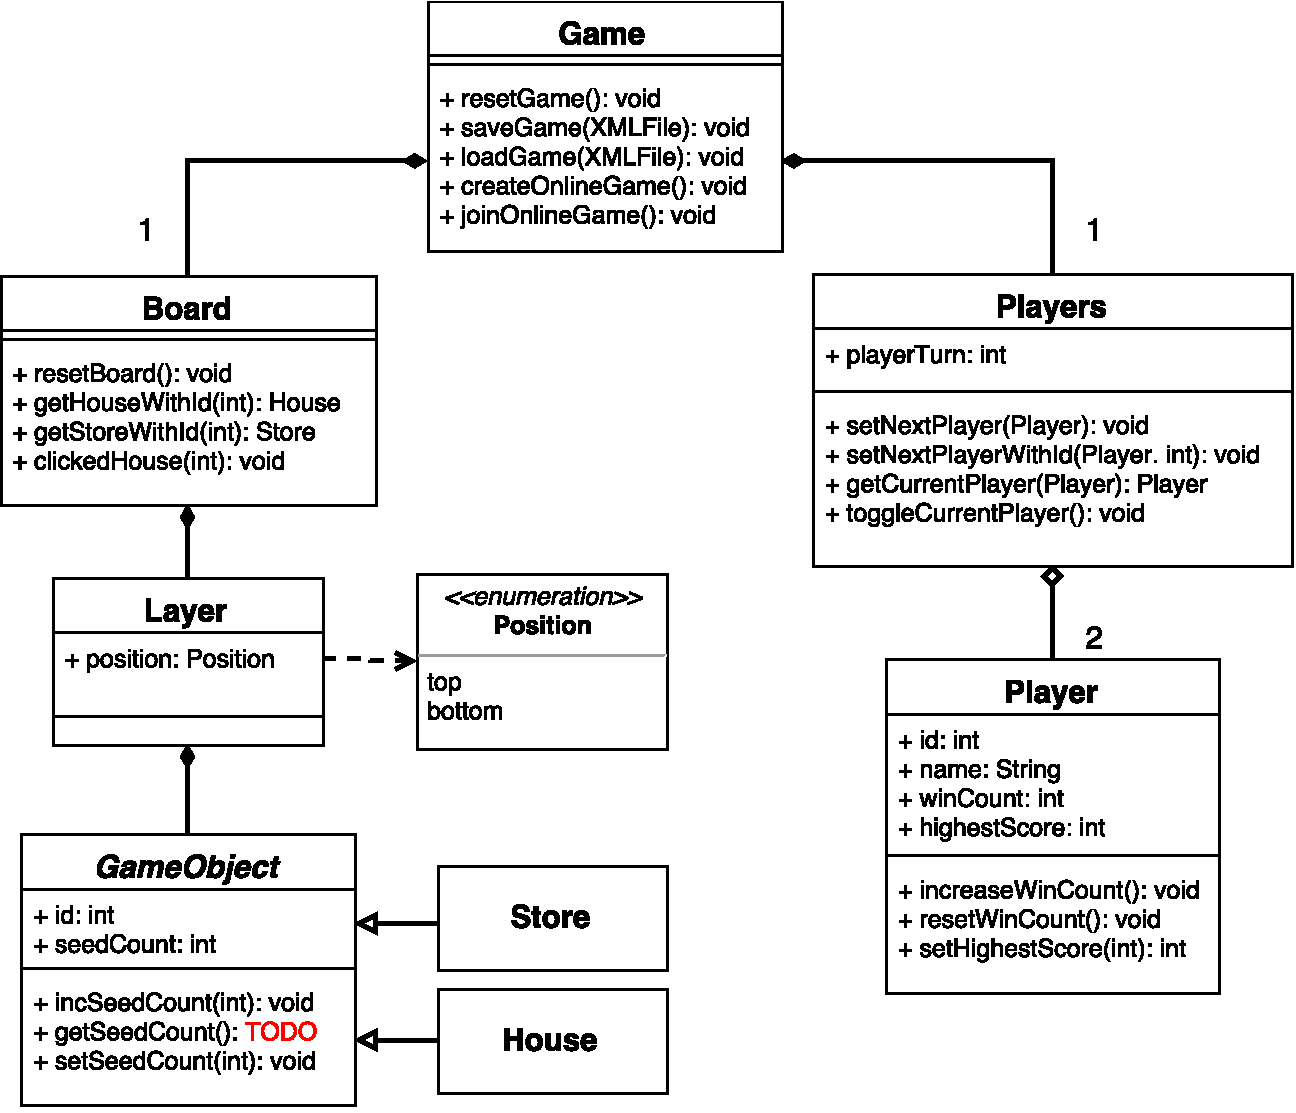
\includegraphics[scale=0.32]{./../Diagrams/ClassDiagram.pdf}
\end{center}
\end{frame}

\section{Demo}
\begin{frame}
\frametitle{Outline}
\begin{enumerate}
\item Mancala
\item Technologien
\item Architektur
\item UML
\item \textbf{Demo}
\item Probleme
\end{enumerate}
\end{frame}

\begin{frame}[plain, c]
\begin{center}
\Large Demo
\end{center}
\end{frame}

\section{Problems}
\begin{frame}
\frametitle{Outline}
\begin{enumerate}
\item Mancala
\item Technologien
\item Architektur
\item UML
\item Demo
\item \textbf{Probleme}
\end{enumerate}
\end{frame}

\begin{frame}
\frametitle{Probleme}

\end{frame}

\section{Questions}
\begin{frame}[plain, c]
\begin{center}
\Large Fragen?
\end{center}
\end{frame}

\end{document}
